% !TEX program = xelatex
\documentclass{iopjournal}

% ── 宏包（iopjournal.cls 已加载 graphicx, xcolor, hyperref）──
\usepackage{amsmath,amssymb}
\usepackage{booktabs}
\usepackage{multirow}
\usepackage{algorithm}
\usepackage{algpseudocode}
\usepackage{siunitx}
\usepackage[caption=false]{subfig}
\usepackage{xeCJK}

% ── CJK 字体 ──────────────────────────────────────────────────
\setCJKmainfont{Noto Serif CJK SC}
\setCJKsansfont{Noto Sans CJK SC}
\setCJKmonofont{Noto Sans CJK SC}

\graphicspath{{media/}}
\sisetup{round-mode=places, round-precision=3}

% ── 自定义命令 ─────────────────────────────────────────────────
\newcommand{\ie}{\textit{i.e.}}
\newcommand{\eg}{\textit{e.g.}}
\newcommand{\etal}{\textit{et al.}}

\begin{document}

\articletype{Paper}

% ══════════════════════════════════════════════════════════════
\title{CNN-PDDQN：一种改进的面向森林场景的UGV深度强化学习运动规划方法}

\author{Firstname Lastname$^1$, Firstname Lastname$^2$ and Firstname Lastname$^{2,*}$}

\affil{$^1$Affiliation 1}

\affil{$^2$Affiliation 2}

\affil{$^*$Author to whom any correspondence should be addressed.}

\email{e-mail@e-mail.com}

\keywords{traversability, Ackermann UGV, deep reinforcement learning, motion planning}

% ══════════════════════════════════════════════════════════════
\begin{abstract}
森林巡检与作业要求自主地面无人车（UGV）在树干密集、地形起伏的非结构化环境中，实时生成满足运动学约束的安全可执行轨迹。针对传统图搜索与采样规划在狭窄通道中计算开销大、轨迹可控性不足的问题，提出一种面向森林场景的深度强化学习运动规划方法。首先利用FAST-LIO2构建先验三维点云地图，并基于可通行性评估生成二维占据栅格及到目标的代价场；随后将规划过程建模为马尔可夫决策过程，设计基于CNN-PDDQN的策略学习框架，并结合双圆足迹碰撞近似与进度/平滑约束构造奖励函数。推理阶段引入在线动作掩码与短视滚动预测的可行域过滤，剔除必碰撞或低收益动作，并配合回退机制与分层验证以降低无效动作选择与振荡风险。随机森林仿真与真实林地实验表明，该方法在路径质量与规划效率之间取得更优折中：仿真长路径任务平均规划耗时为0.337\,s，真实林地场景平均规划耗时为0.185\,s，均显著低于传统算法；同时生成路径更短，验证了所提方法在森林环境中的实时性与可执行性优势。
\end{abstract}

% ══════════════════════════════════════════════════════════════
\section{介绍}\label{sec:intro}

近年来，随着林地巡检、生态监测及林下资源作业等任务需求的增加，地面无人车（UGV）在森林等非结构化环境中的自主通行能力面临着严峻挑战。与城市道路等具备清晰几何特征的结构化场景显著不同，林间环境通常具有地表起伏剧烈、障碍物（如树干）分布密集且无规则等特点。在这一复杂条件下，路径规划算法面临着双重压力：一方面需要在障碍物稠密的区域生成严格无碰撞的安全轨迹，另一方面需在极有限的狭窄间隙中实现灵活穿梭。这种对安全性与通过性的双重追求，运动规划算法的计算成本成为一大难题。

现有的运动规划算法大致可分为三类：（1）传统算法；（2）优化算法；（3）基于强化学习的算法。

\subsection{传统规划方法}

传统规划方法在工程上应用广泛，包括基于图的方法和基于采样的方法等等。传统方法优点是原理成熟，缺点是路径易不连续、易陷局部最优、计算效率有限。

其中，基于图搜索的方法中，Hybrid\,A*由于能够在搜索扩展过程中同步完成碰撞检测、并严格满足车辆（或车类机器人）运动学约束而被广泛采用。Jiang等人\cite{jiang2025hybrid}面向果园窄通道贴行导航，构建了``改进D*~Lite全局规划+窄段Hybrid\,A*局部重规划+轨迹平滑''的混合框架，从而在安全贴行与可执行性之间取得折中。Lian等人\cite{lian2023trajectory}针对狭窄环境代客泊车，先以增强Hybrid\,A*生成高质量初值，再引入非线性最优控制进行二次优化，以在受限空间内获得更可行、更平滑的泊车轨迹。Pang等人\cite{pang2022curvature}在自动泊车场景中提出基于Hybrid\,A*的反向搜索与碰撞剪枝策略，在保证曲率连续与终端精度的同时提升规划效率。Thoresen等人\cite{thoresen2021path}将地形可通行性评估融入Hybrid\,A*代价函数，使UGV在复杂地形上更倾向于选择风险更低、可通过性更强的路径。Zhang等人\cite{zhang2024twostage}面向露天矿大尺度场景提出两阶段二分Hybrid\,A*，通过障碍多边形化以及对转向角/步长的二分搜索，降低扩展冗余并加速规划。总体而言，图搜索算法能够较高效地给出可行路线，但在长路径下搜索过程中引入碰撞检测，往往会显著增加计算开销，进而导致规划用时过长等局限。

基于采样的规划方法通常以PRM、RRT及其改进RRT*为代表，通过在配置空间进行随机采样、并以图结构增量扩展搜索，从而在高维场景中高效获得可行路径。面向越野/非结构化环境中``植被遮挡导致地形难感知、地形不确定导致通行性难保证、风险难以显式量化、可靠性评估代价高''等问题，研究者普遍在RRT*框架上引入地形推断、可靠性约束与风险引导等机制：Jian等人\cite{jian2024path}提出PE-RRT*，将支撑平面估计与RRT*的采样/扩展过程紧密耦合，并据此实现植被遮挡地形下的实时、可行且更安全的路径生成；Jiang等人\cite{jiang2022r2rrt}提出R2-RRT*，在RRT*搜索过程中显式引入不确定地形条件下的可靠性指标（如任务机动可靠度MMR）作为约束/评价准则，以获得更鲁棒的越野任务规划结果；Tian等人\cite{tian2023driving}提出PF-RRT*（势引导的RRT*），通过势场对障碍物与越野风险进行连续表征，并在采样偏置与代价设计中实现安全性与效率的权衡；Yin等人\cite{yin2023efficient}则在RRT*框架中耦合替代模型以近似可靠性评估、减少高代价仿真调用，从而提升越野可靠性路径规划的整体计算效率。

\subsection{基于优化的算法}

基于优化的算法主要包括遗传算法（GA）、蚁群优化算法（ACO）、粒子群算法（PSO）以及人工蜂群算法（ABC）等，这类方法通常通过构建目标函数与约束、并借助群体智能的迭代搜索，在复杂环境中获得近似最优路径。围绕多机器人协同、非完整约束车辆的可跟踪性、以及栅格环境的搜索效率等问题，相关研究多从``改进单一优化器''与``混合多种群智能''两条思路展开：Cai等人\cite{cai2024cooperative}面向分布式多移动机器人协同场景，提出一种基于优化ACO的合作路径规划方法，并通过改进搜索与信息素更新机制，以提升多机器人规划的协同性与整体效率。Huo等人\cite{huo2024smooth}面向Ackermann转向移动机器人，提出改进ACO结合B样条曲线的平滑规划思路，并将路径平滑与可跟踪需求纳入优化过程，以获得更连续、可执行的运动轨迹。Li等人\cite{li2023mixing}将ACO与ABC进行混合设计，用于求解移动机器人路径规划问题，并利用两者在探索/开发上的互补性，以兼顾全局搜索能力与局部寻优效果。Xu等人\cite{xu2022quartic}引入四次Bezier过渡曲线并结合改进PSO，构建面向平滑路径的优化求解框架，并以曲率高阶连续与转向过渡约束为核心，以改善路径连续性与转弯过渡质量。Yildirim和Akay\cite{yildirim2025efficient}在栅格地图框架下设计改进ABC算法用于路径规划，并引入路径线性化与局部搜索等机制，以减少不必要拐角、提升网格环境中的搜索效率与路径质量。

\subsection{基于强化学习的方法}

基于强化学习（RL）的路径规划方法通常以Q-learning或SARSA等时序差分方法，以及DQN等深度强化学习为代表，其核心是通过与环境交互学习状态---动作价值，从而获得导航策略；围绕``鲁棒性、可扩展性、可解释的评价机制、以及非结构化场景适应性''等目标，相关工作大多在价值函数表示、奖励/评价设计与启发式先验融合上做文章：Kumar等人\cite{kumar2025dsqn}提出DSQN（DeepSpiking Q-Network），将脉冲神经元机制引入深度Q学习框架，并在同一决策过程中融合全局目标与局部观测信息，以提升移动机器人路径规划的鲁棒性与综合性能；Li和Wang\cite{li2025iqaco}将Q评估机制显式融入ACO，提出改进的IQACO，以Q值驱动的节点评价替代/弱化传统信息素主导的判断，并缓解参数敏感与搜索稳定性问题，从而提升规划质量与收敛表现；Maoudj和Hentout\cite{maoudj2020optimal}基于Q-learning构建最优路径规划框架，并通过更高效的学习策略设计，在保证无碰撞与最优性的同时尽量缩短求解时间；Sichkar\cite{sichkar2019reinforcement}则围绕移动机器人全局路径规划任务，对Q-learning与SARSA等强化学习算法的实现与效果差异进行对比分析，并从学习效率与路径生成特性等角度给出经验性结论；Xu等人\cite{xu2026rl}提出强化学习驱动的启发式路径规划思路，面向非结构化环境中的自动化特种车辆需求，利用传统启发式先给出初始规划结果、再由RL进行调整优化，以避免纯RL在早期学习阶段的低效与不稳定；Zhou等人\cite{zhou2018dqn}设计基于DQN的移动机器人路径规划方法，通过训练网络逼近动作价值函数，并据此在密集环境中选择动作序列以获得有效的全局路径。然而，将RL直接应用于森林狭窄通道规划仍存在突出困难：其一，阿克曼车辆的非完整约束与近障安全距离约束会导致离散动作集合中大量动作在当前状态下不可行，若缺少约束处理机制，策略容易选择``Q值看似较高但实际不可执行''的动作，引发碰撞、振荡或效率下降；其二，在非结构化环境中可通行区域提取容易受地表起伏、落叶堆积、点云稀疏及噪声影响，若生成的地图或可通行性估计不可靠，学习策略难以稳定收敛并保证安全。

\subsection{本文贡献}

针对上述问题，本文提出一套面向森林非结构化狭窄障碍场景的UGV运动规划框架，主要贡献如下：

\begin{enumerate}
  \item 提出一套``先验点云建图---可通行性分割---二维占据栅格/代价场构建---运动规划''的完整流程，面向森林非结构化地形提高可通行区域提取与规划输入的可靠性。
  \item 提出基于CNN-PDDQN的UGV运动规划策略，并结合两圆足迹与代价场设计，将安全裕度、进度与可控性约束统一纳入MDP建模与奖励函数中，实现可执行的学习型规划。
  \item 提出面向狭窄障碍场景的在线动作掩码与可行域过滤机制，通过短视预测筛除低收益动作，降低策略选择无效动作的概率，从而提升规划稳定性与实时性。
  \item 在多场景仿真与真实林地实验中验证了方法的有效性。
\end{enumerate}

本文其余部分组织如下：第二节介绍系统总体框架与关键方法，包括点云建图、可通行性分割、代价场构建、MDP建模、CNN-PDDQN策略与动作掩码机制；第三节给出仿真与真实场景下的对比实验结果与讨论；第四节总结全文并展望后续工作。

% ══════════════════════════════════════════════════════════════
\section{方法}\label{sec:method}

如图~\ref{fig:framework}所示，本文提出一种面向森林场景的UGV路径规划框架，整体流程分为三个阶段。第一阶段，利用FAST-LIO2算法融合激光雷达与IMU数据，构建先验三维点云地图；第二阶段，对点云地图进行可通行性评估与分割，将三维几何信息投影为二维占据栅格地图；第三阶段，在规划过程中，针对阿克曼车辆的非完整约束与狭窄障碍环境，设计了CNN-PDDQN深度强化学习策略在格栅地图进行路径规划。（第三阶段写的不好）

\begin{figure}[t]
\centering
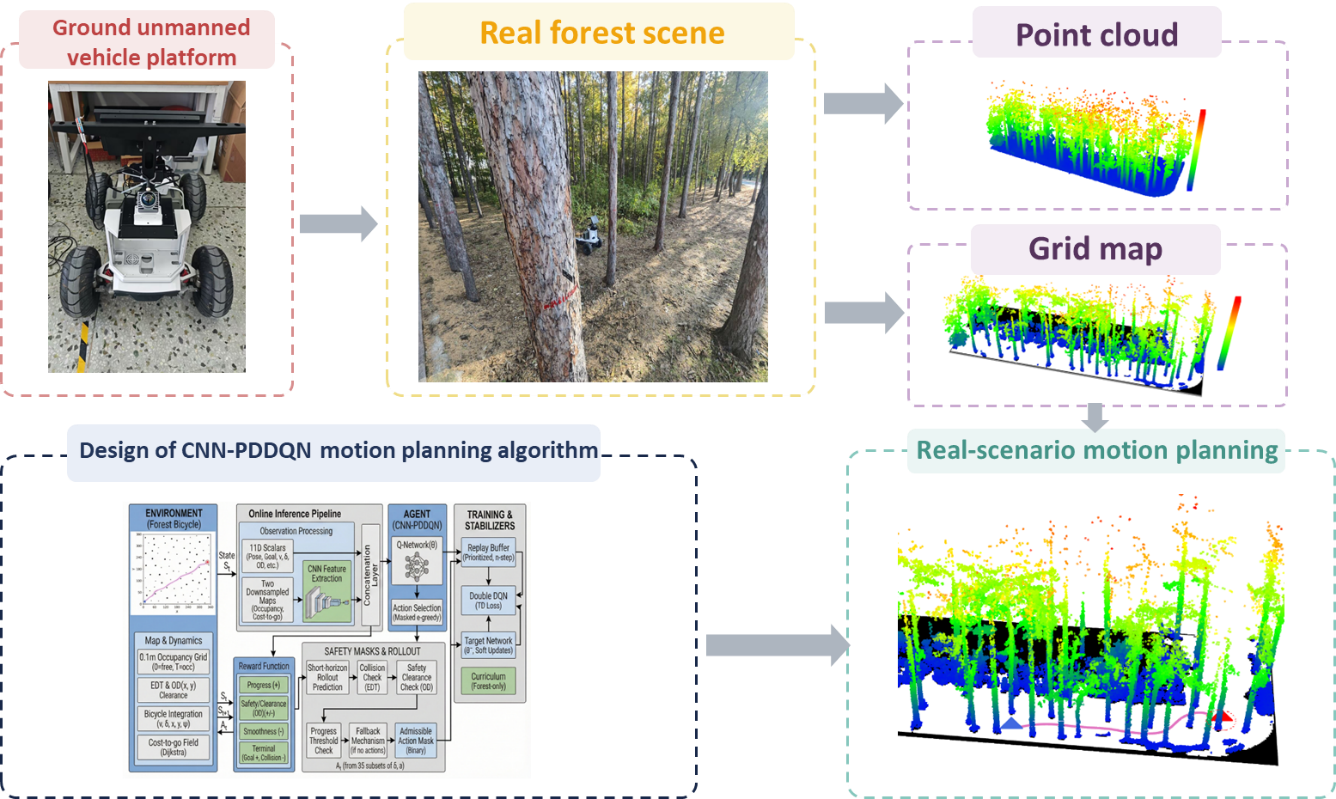
\includegraphics[width=\columnwidth]{image1.png}
\caption{面向森林场景的UGV运动规划框架}
\label{fig:framework}
\end{figure}

\subsection{地面无人车与传感器}

实验平台采用阿克曼转向的地面无人车（UGV），如图~\ref{fig:platform}所示。底盘为前轮转向、后轮驱动的阿克曼结构，配备充气轮胎与减震悬架以适应林间起伏地形。感知传感器为Livox~Mid-360三维激光雷达，内置IMU，以30°俯角安装于车体前方，提供360°视场角与最远100\,m的测距能力。车载计算单元为Jetson AGX Orin，运行Ubuntu 20.04与ROS1 Noetic，负责SLAM建图与路径规划的在线计算。

\begin{figure}[t]
\centering
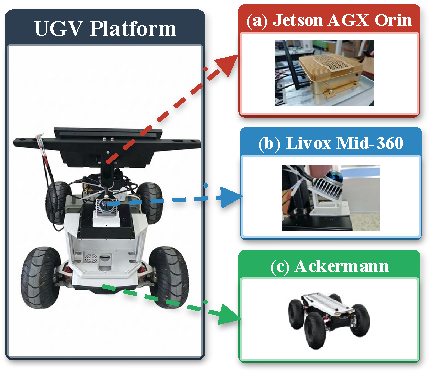
\includegraphics[width=0.55\columnwidth]{fig2_platform.pdf}
\caption{地面无人车实验平台}
\label{fig:platform}
\end{figure}

\subsection{基于FAST-LIO2的先验点云地图的建立}

先验三维点云地图的建立依赖于同步定位与建图（SLAM）技术，即在未知环境中同步估计传感器位姿并构建环境地图。本文采用FAST-LIO2作为SLAM框架\cite{xu2022fastlio2}，该框架基于高效的紧耦合迭代卡尔曼滤波器，具有两项核心设计：一是跳过手工特征提取步骤，直接将原始点云配准到地图，从而能够利用环境中的细微几何特征提高定位精度；二是采用增量式k-d树（ikd-Tree）维护局部地图，支持点的增量插入、删除与动态重平衡，在保持地图实时更新的同时显著降低计算开销。在建图过程中，根据估计的运动对单次扫描内点云进行去畸变，并将各帧点云通过刚体变换统一到全局坐标系下进行增量拼接，生成三维点云先验地图。

将第$k$帧点云表示为集合$\mathcal{P}_{k} = \{p_{k,i}\}_{i=1}^{N_k}$，其中$p_{k,i} = [x_{k,i},y_{k,i},z_{k,i}]^\mathsf{T}$定义于激光雷达坐标系。FAST-LIO2输出该帧在全局坐标系下的位姿可表示为刚体变换$T_k = [R_k, t_k]$，其中$R_k \in SO(3)$为旋转矩阵，$t_k \in \mathbb{R}^{3}$为平移向量。点云由激光坐标系变换到全局坐标系的关系为：
\begin{equation}
  p_{k,i}^{g} = R_k\, p_{k,i} + t_k
\end{equation}
其中$p_{k,i}^{g}$为全局坐标系下的点坐标。所有变换后的点集$\{p_{k,i}^{g}\}$被增量式地融合至全局地图中。

在点云地图建立后，对其进行体素降采样以降低点云密度、减少后续计算量，并施加统计离群点移除滤波（SOR）以滤除传感器噪声产生的离群点，得到适用于后续可通行性分析的干净点云地图。

\subsection{基于可通行评估的点云分割}

在获取干净的点云地图后，需要从中分割出可通行区域，作为后续路径规划的输入。传统方法多依赖几何高度差或简单阈值进行障碍物检测，但在森林等非结构化环境中，由于地表起伏、落叶堆积、点云稀疏及传感器噪声等因素，容易造成可通行区域的误判。本文使用基于可通行性分析的点云分割方法，将三维点云先验地图投影为二维占据栅格地图，为后续路径规划提供基础\cite{feng2025constraint}。


给定全局坐标系下的点云地图$\mathcal{M} = \{\mathbf{p}_i\}_{i=1}^{N}$，其中$\mathbf{p}_i = [x_i, y_i, z_i]^\top$。首先剔除高度$z_i > z_{\max}$的点以排除与地面通行无关的结构。对每个保留点$\mathbf{p}_i$，取半径$r$内的邻域$\mathcal{N}_r(\mathbf{p}_i)$，逐一计算与邻域点$\mathbf{p}_j$之间的坡度角：
\begin{equation}
  \theta_{ij} = \arctan\!\left(\frac{|z_i - z_j|}{\sqrt{(x_i-x_j)^2+(y_i-y_j)^2}}\right)
\end{equation}
若地面无人车最大爬坡角为$\theta_{\max}$，则$\theta_{ij} > \theta_{\max}$意味着$\mathbf{p}_i$到$\mathbf{p}_j$方向不可通行。但林地地面常有落叶、碎石覆盖，直接用硬阈值判定会造成大量误判。为此引入松弛因子$\lambda \in [0,1]$，统计邻域内超限点的比例：
\begin{equation}
  r_{\text{slope}} = \frac{1}{|\mathcal{N}(\mathbf{p}_i)|}\sum_{\mathbf{p}_j \in \mathcal{N}(\mathbf{p}_i)} \mathbb{I}(\theta_{ij} > \theta_{\max})
\end{equation}
其中$\mathbb{I}(\cdot)$为指示函数。当$r_{\text{slope}} \leq \lambda$时，虽然局部地形存在粗糙起伏，但超限点占比尚在容许范围内，将$\mathbf{p}_i$标记为可通行；反之标记为不可通行。

\subsection{地面无人车路径规划}

\subsubsection{车辆参数与运动学建模}


本文采用等效自行车模型描述阿克曼转向车辆的非完整运动约束，如图~\ref{fig:kinematics}所示：(a)为运动学模型示意，(b)标注了实验平台的轴距$L$与外形尺寸等关键几何参数。以后轴中心为参考点，车辆状态为$s=(x,y,\theta)$，其中$(x,y)$为位置，$\theta$为航向角；控制输入为$u=(v,\delta)$，其中$v$为后轴纵向速度，$\delta$为前轮转角。在低速纯滚动无侧滑假设下，运动学方程为：
\begin{equation}
  \begin{aligned}
    \dot{x} &= v\cos\theta \\
    \dot{y} &= v\sin\theta \\
    \dot{\theta} &= \frac{v}{L}\tan\delta
  \end{aligned}
\end{equation}

\begin{figure}[t]
\centering
\subfloat[(a)]{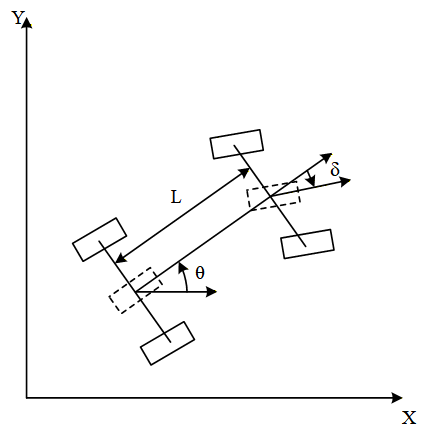
\includegraphics[width=0.48\columnwidth]{image3.png}}
\hfill
\subfloat[(b)]{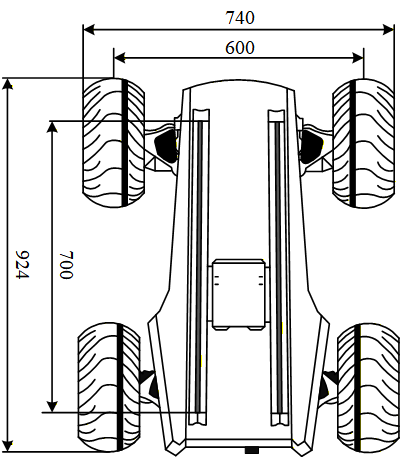
\includegraphics[width=0.48\columnwidth]{image4.png}}
\caption{地面无人车运动学模型与实验平台几何参数}
\label{fig:kinematics}
\end{figure}

\subsubsection{碰撞检测}

如图~\ref{fig:dual_circle}所示，本文采用双圆足迹近似车体轮廓：沿车体纵轴布置两个半径为$r$的圆，分别覆盖前、后关键区域。为高效获取任意位置到最近障碍物的距离，环境预先对占据栅格地图计算欧几里得距离变换（Euclidean Distance Transform），生成全局障碍物距离场。碰撞检测时，仅需在该距离场中查询两圆心所在栅格的距离值$d_1$、$d_2$，当满足以下条件时判定为碰撞：
\begin{equation}
  \min(d_1,\, d_2) \leq r
\end{equation}
相比矩形足迹的多边形相交检测，双圆足迹结合预计算距离场将碰撞判定简化为两次常数时间的查表与比较操作，显著降低了在线规划的计算开销。

\begin{figure}[t]
\centering
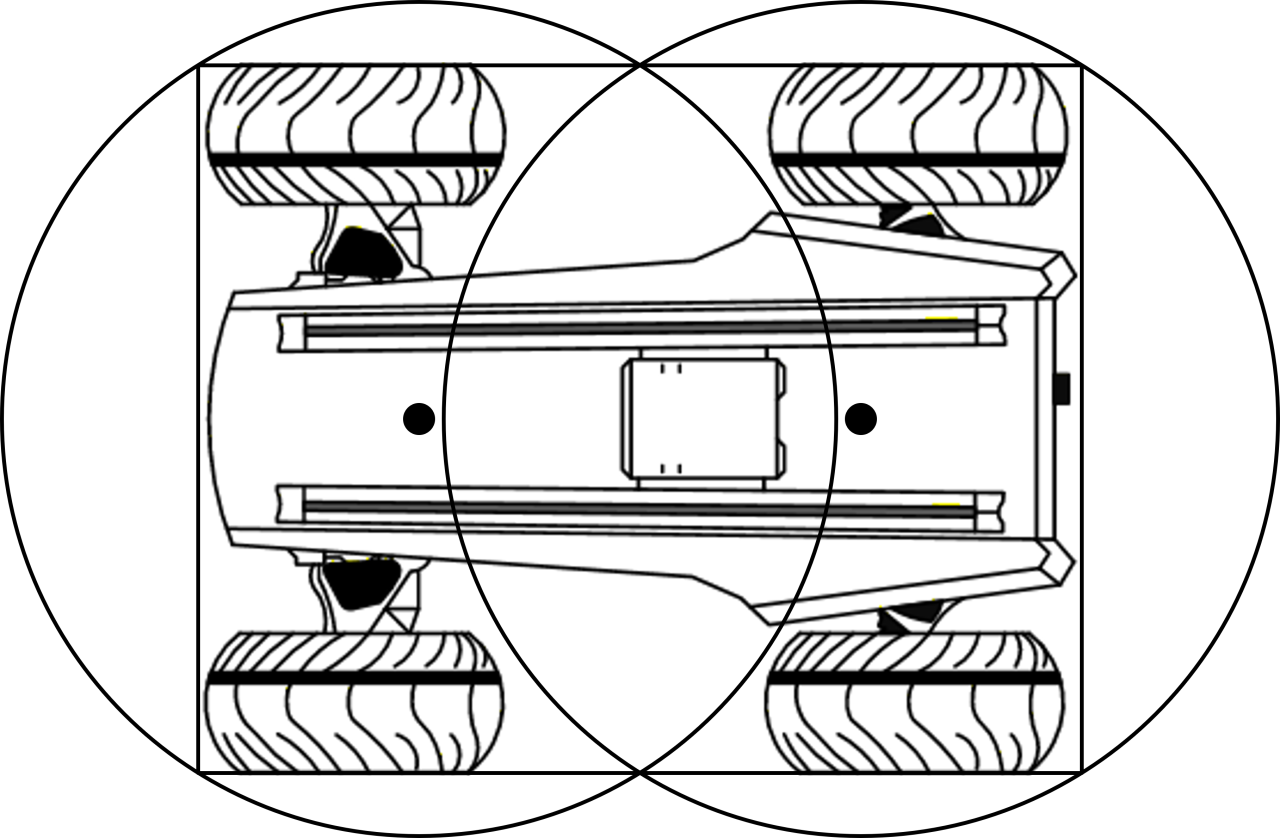
\includegraphics[width=0.55\columnwidth]{image5.png}
\caption{车辆双圆足迹近似示意图}
\label{fig:dual_circle}
\end{figure}

\subsubsection{马尔可夫决策过程（MDP）建模}

MDP可以表示为一个四元组$M=(S,A,P,R)$，其中$S$代表环境中存在的有限状态集，$S_t$代表$t$时刻的状态，$A$表示地面无人车执行的动作，$A_t$表示$t$时刻执行的动作，$P$是转移概率，$R$是奖励函数。基于观察到的环境状态$s_t$，地面无人车随机选择并执行动作$A_t$。随后，环境为地面无人车提供奖励$R_{t+1}$，同时将状态从$S_t$更新为下一个状态$S_{t+1}$。

\paragraph{（1）状态空间}

在状态空间中，三维环境的特征信息被映射到等大小的二维网格中使地面无人车能够在二维格栅网格环境中进行路径规划。根据环境中障碍物的分布，障碍物用黑色网格表示，地面无人车可通行域用白色表示，每个格栅地图的分辨率为0.1\,m。

\paragraph{（2）动作空间}

首先构造一个动作查找表$\mathbf{T}\in\mathbb{R}^{35\times2}$，每个动作对应一组$[\dot{\delta},\, a]$。动作空间可表示为两个离散集合的笛卡尔积：
\begin{equation}
  A = \{(\dot{\delta}_i, a_j) \mid \dot{\delta}_i \in \Delta_{\dot{\delta}},\, a_j \in \Delta_a\},\quad |A|=7\times5=35
\end{equation}
其中转向角速度离散集合为：
\begin{equation}
  \Delta_{\dot{\delta}} = \left\{-\dot{\delta}_{\max},\, -\tfrac{2}{3}\dot{\delta}_{\max},\, -\tfrac{1}{3}\dot{\delta}_{\max},\, 0,\, \tfrac{1}{3}\dot{\delta}_{\max},\, \tfrac{2}{3}\dot{\delta}_{\max},\, \dot{\delta}_{\max}\right\}
\end{equation}
纵向加速度离散集合为：
\begin{equation}
  \Delta_a = \left\{-a_{\max},\, -\tfrac{1}{2}a_{\max},\, 0,\, \tfrac{1}{2}a_{\max},\, a_{\max}\right\}
\end{equation}
其中，$\dot{\delta}_{\max}=60^\circ/\text{s}$，$a_{\max}=1.5$\,m/s$^2$，并且时间步长$dt=0.05$\,s、最大速度$v_{\max}=2.0$\,m/s、最大转向角$\delta_{\max}=27^\circ$。

在训练和推理时，策略网络输出的离散动作通常用整数索引表示：
\begin{equation}
  a_t \in \{0, 1, \ldots, 34\}
\end{equation}
并通过查表映射为连续控制对$(\dot{\delta}_t, a_t)$。

\paragraph{（3）奖励函数的设计}

运动学模型状态量为$s_t = (x_t, y_t, \theta_t)$，控制量为$v_t, \delta_t$，动作为转向角速度与纵向加速度。奖励在整体可写为：
\begin{equation}
  R_t = r_{\text{prog}} + r_{\text{time}} + r_{\text{smooth}} + r_{\text{safety}} + r_{\text{term}}
\end{equation}

\textit{A.~进度奖励}

为避免只在终点给奖励导致的稀疏问题，环境优先使用清障代价的下降量作为进度，令$C(s)$为考虑绕障的代价场，则：
\begin{equation}
  r_{\text{prog}} = k_p(C(s_t) - C(s_{t+1}))
\end{equation}
当代价场不可用或者非有限时，回退为欧氏目标距离$D(s)$的下降量：
\begin{equation}
  r_{\text{prog}} = k_p(D(s_t) - D(s_{t+1}))
\end{equation}
该代价场建立在预计算的距离场与可通行区域上：环境先计算每个栅格到障碍/边界距离，并将边界视作障碍，之后用``最小无碰撞清障阈值''用于代价场的建立。

\textit{B.~时间惩罚}

为每步施加常数时间惩罚，鼓励更快完成路径规划算法：
\begin{equation}
  r_{\text{time}} = -k_t
\end{equation}

\textit{C.~平滑与可控性约束奖励}

为避免策略在狭窄通道出现转向抖动、频繁急加减速，引入控制平滑项与曲率惩罚：
\begin{equation}
  r_\delta = -k_\delta(\delta_{t+1}-\delta_t)^2
\end{equation}
为解决加速度平滑问题，惩罚$a_t$相对前一时刻的变化，并按速度比例缩放，避免从静止起步被过度惩罚：
\begin{equation}
  r_a = -k_a(a_t - a_{t-1})^2\left(\frac{v_{t+1}}{v_{\max}}\right)^2
\end{equation}
对于大转角/大曲率惩罚，用$\tan(\delta)$表示曲率趋势：
\begin{equation}
  r_\kappa = -k_\kappa \tan^2(\delta_{t+1})
\end{equation}

\textit{D.~安全无碰撞奖励}

环境采用``两圆足迹''近似车体：取两圆心到最近障碍边界距离$d_1, d_2$，圆半径为$r$，则：
\begin{equation}
  OD(s) = \min(d_1 - r,\, d_2 - r)
\end{equation}
\begin{equation}
  \text{collision} \Leftrightarrow (d_1 \leq r) \vee (d_2 \leq r)
\end{equation}
若未处于碰撞状态且$OD < d_s$（安全距离），则采用``反距离差''构造惩罚，并对惩罚幅值做上限截断：
\begin{equation}
  r_{\text{obs}} = -\min\!\left(k_{\text{obs,max}},\, k_o\!\left(\frac{1}{OD+\varepsilon}-\frac{1}{d_s+\varepsilon}\right)\right),\quad OD < d_s
\end{equation}

当$OD < d_v$时，额外惩罚``在近障区域仍保持较高速度''的行为：
\begin{equation}
  r_v = -k_v\left(\frac{d_v - OD}{d_v}\right)\left(\frac{v_{t+1}}{v_{\max}}\right)^2
\end{equation}
同时引入``软速度上限''：
\begin{equation}
  v_{\text{cap}} = v_{\max} \cdot \text{clip}\!\left(\frac{OD}{d_v}, 0, 1\right),\quad
  r_{\text{cap}} = -k_c \cdot \max(0, v_{t+1} - v_{\text{cap}})^2
\end{equation}

\subsubsection{基于CNN-PDDQN的深度强化学习路径规划策略}

在MDP建模基础上，本文采用CNN对局部占据栅格/代价图进行特征提取，并以CNN-PDDQN学习离散动作的价值函数，实现端到端的路径规划决策。训练阶段结合Double DQN缓解价值过估计，并引入优先经验回放提升学习效率；在线推理时通过安全动作掩码约束动作输出，整体流程如图~\ref{fig:cnn_pddqn}所示。

\begin{figure}[t]
\centering
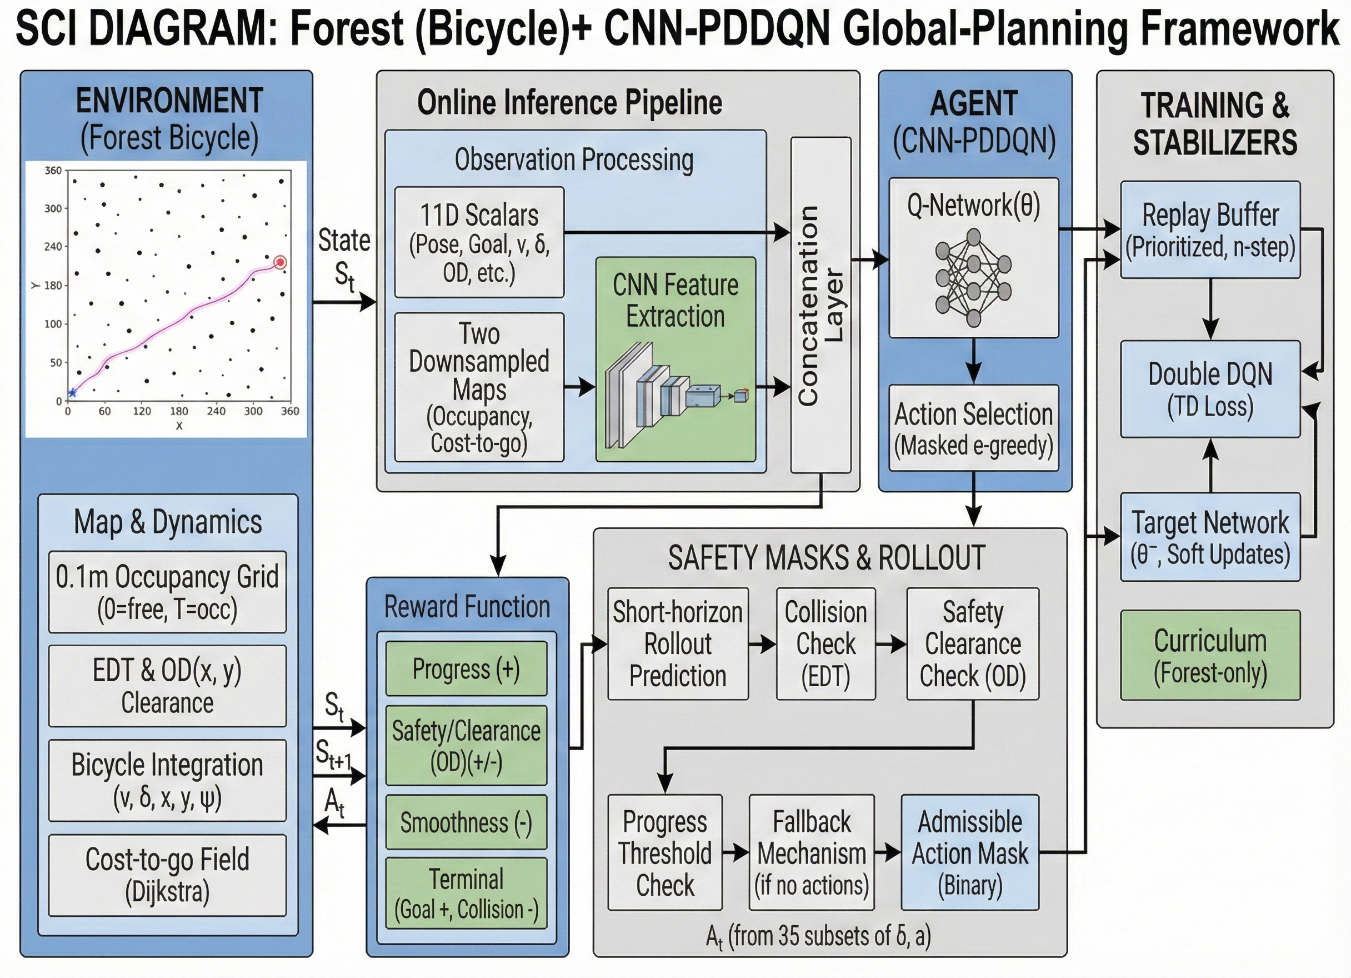
\includegraphics[width=\columnwidth]{image6.png}
\caption{CNN-PDDQN路径规划策略的在线推理与训练框架}
\label{fig:cnn_pddqn}
\end{figure}

\paragraph{（1）CNN深度神经网络}

\textit{A.~输入表示与结构化融合}

为使网络同时``感知''全局可通行结构与到目标的代价信息，环境观测被统一编码为一个扁平向量：其前11维为低维标量状态（包含归一化后的智能体/目标位置、航向用$\sin\theta, \cos\theta$的连续表示、速度与转角的归一化量、基于足迹的代价场归一化量、目标相对方位角以及与障碍/边界相关的安全余量等），用于提供动力学与目标条件信息；其余部分为两张大小为$N \times N$的全局栅格图按通道展平后的拼接，其中占据栅格由静态障碍物网格通过最近邻下采样得到并线性映射到$[-1,1]$，代价场栅格先对代价进行上界截断与$[0,1]$归一化，再用面积插值下采样并同样映射到$[-1,1]$。因此观测维度满足$D = 11 + 2N^2$，与环境的约束一致。实际送入CNN时，网络并不直接对整个向量卷积，而是将向量后段重排为$\mathbf{M} \in \mathbb{R}^{2 \times N \times N}$的``二通道地图张量''做卷积特征提取，同时将前11维标量作为旁路特征在后续与卷积特征拼接，从而实现``全局地图（CNN）+低维状态（标量）''的结构化融合。

\textit{B.~CNN-Q网络结构}

CNN编码器由3层2D卷积与ReLU组成（无池化层，以步长实现下采样）：

\begin{table}[t]
\centering
\caption{CNN编码器结构参数}
\label{tab:cnn_structure}
\footnotesize
\begin{tabular}{@{}ccccc@{}}
\toprule
\textbf{层} & \textbf{卷积核} & \textbf{stride} & \textbf{padding} & \textbf{输出通道} \\
\midrule
Conv1 & $3\times3$ & 1 & 1 & 32 \\
Conv2 & $3\times3$ & 2 & 1 & 64 \\
Conv3 & $3\times3$ & 2 & 1 & 64 \\
\bottomrule
\end{tabular}
\end{table}

该CNN相当于学习一个从``代价场''到``高层空间语义特征''的非线性映射：
\begin{equation}
  \phi_\theta: \mathbb{R}^{2 \times N \times N} \rightarrow \mathbb{R}^{d_{\text{cnn}}}
\end{equation}
其中$d_{\text{cnn}}$由卷积输出的展平长度决定。

\textit{C.~Q值读出}

最终Q函数以拼接特征为输入输出35维动作价值向量：
\begin{equation}
  \mathbf{Q}(s, \cdot) = f_\theta(\mathbf{h}) \in \mathbb{R}^{35}
\end{equation}
实现上这是一个可配置深度的全连接``读出头''，其输入维度为$11 + d_{\text{cnn}}$，输出维度为35。

\paragraph{（2）自适应动作选择策略}

在森林等场景中，阿克曼车辆的非完整约束与近障安全距离约束会导致离散动作集合$A$中大量动作在当前状态下不可行：部分动作在短时间内必然碰撞或安全间隙不足，部分动作虽不碰撞但对目标代价几乎无改善，从而引起局部振荡与规划效率下降。为降低$\arg\max_a Q(s_t, a)$及普通$\varepsilon$-greedy在此类状态下选择``高Q但不可执行动作''的概率，本文引入一种在线可行域过滤机制：根据当前状态构造可采纳动作子集，并在该子集上执行掩码化$\varepsilon$-greedy。该策略可视为一种状态相关的动作掩码与安全过滤思想在离散动作规划中的实现。

\textit{A.~短视滚动预测与可采纳判别}

令时刻$t$的状态为$s_t$，离散动作集合为$A = \{a_i\}_{i=1}^{|A|}$。每个离散动作$a_i$通过动作查表映射为连续控制量$u_i = (\dot{\delta}_i,\, a_i)$。对任一候选动作$a_i$，在固定预测步长$H$内保持控制量不变，基于运动学模型对未来状态进行前向积分得到预测轨迹$\hat{x}_{t+1:t+H}^{(i)}$。在滚动预测过程中统计其中碰撞指示$c_i$为若预测区间内任一步满足碰撞判据则$c_i = 1$，否则$c_i = 0$；

最小安全间隙$d_i^{\min}$为预测区间内车辆足迹到最近障碍/边界的最小距离为目标推进量$\Delta J_i$。

目标代价$J(\cdot)$的公式如下：
\begin{equation}
  \Delta J_i = J(x_t) - J(\hat{x}_{t+H}^{(i)})
\end{equation}
据此定义状态相关的可采纳动作集合：
\begin{equation}
  A_{\text{adm}}(s_t) = \{a_i \in A \mid c_i=0,\, d_i^{\min}\geq d_{\text{thr}},\, (\Delta J_i \geq \eta) \vee \text{reached}\}
\end{equation}
其中$d_{\text{thr}}$为最小安全距离阈值，$\eta$为最小推进阈值，reached表示预测终端状态已满足到达目标判据。

\textit{B.~回退机制与近目标退化抑制}

在极端状态下可能出现$A_{\text{adm}}(s_t) = \varnothing$。为保证策略始终可执行，定义仅包含安全约束的集合：
\begin{equation}
  A_{\text{safe}}(s_t) = \{a_i \in A \mid c_i=0,\, d_i^{\min}\geq d_{\text{thr}}\}
\end{equation}
当$A_{\text{adm}}(s_t)$为空时回退到$A_{\text{safe}}(s_t)$。此外，为抑制接近目标时频繁选择制动/倒车导致的退化行为，仅当在同一阈值下不存在任何满足推进条件的前向动作时，才允许将反向动作纳入可选集合。

\textit{C.~掩码化$\varepsilon$-greedy动作选择}

利用掩码后的贪心选择公式为：
\begin{equation}
  a_t = \arg\max_{a_i \in A}\bigl(Q_\theta(s_t, a_i) + (1 - m_i) \cdot (-\infty)\bigr)
\end{equation}
即将不可采纳动作的Q值置为极小，从而在推理阶段严格排除不满足约束的动作；探索阶段则在可采纳集合中均匀采样实现$\varepsilon$-greedy。该``掩码化选择''是无效动作屏蔽的常用实现方式。

\textit{D.~计算开销与分层验证}

全量掩码的最坏计算复杂度为$O(|A|H)$。为降低平均开销，本文采用分层验证：优先检验无掩码贪心动作；若不可采纳，仅对Q值前$k$的候选动作进行逐一可采纳性验证；仅当上述步骤均失败时才计算全量掩码并在掩码下重新贪心，从而在保证安全性的同时减少在线计算。

\paragraph{（3）算法流程}

所提出CNN-PDDQN的训练与在线规划流程，以伪代码形式总结于算法~\ref{fig:algorithm}。CNN-PDDQN以卷积神经网络对下采样后的全局栅格观测进行编码，输出离散动作集合上的动作价值函数$Q_\theta(s,a)$。为提升值函数学习的稳定性与减小过估计偏差，本文采用Double DQN的目标构造：由在线网络执行动作选择、由目标网络执行价值评估，从而解耦``$\max$''算子中的选择与估计过程。

进一步地，为在稀疏奖励与长时域决策下提升样本效率，采用$n$-step回报来构造TD目标：对从时刻$t$开始的$n$步奖励进行折扣累计，并在未终止时引入自举项。该做法在DQN系列改进中被广泛使用。

考虑到复杂障碍环境下离散动作空间中存在大量短视必碰撞/越界或对目标推进贡献极小的动作，本文在决策层引入动作屏蔽：对每个候选动作进行短时域滚动预测与几何可行性判定，得到可采纳动作集合$A_t \subseteq A$。随后仅在$A_t$内执行掩码化$\varepsilon$-greedy选择，从而在推理阶段显式排除不安全动作，并在训练阶段减少无效探索。

目标网络采用Polyak平均（软更新）进行平滑跟踪：
\begin{equation}
  \bar{\theta} \leftarrow (1-\tau)\bar{\theta} + \tau\theta
\end{equation}
以降低目标抖动并提升训练稳定性。

对于样本$(s, a, R^{(n)}, s', \text{done}, n)$，Double~DQN的$n$-step~TD目标写为：
\begin{equation}
  a^* = \arg\max_{a' \in A(s')} Q_\theta(s', a'),\quad
  y = \begin{cases} R^{(n)}, & \text{done}=1 \\ R^{(n)}+\gamma^n Q_{\bar{\theta}}(s', a^*), & \text{otherwise} \end{cases}
\end{equation}
并最小化Huber损失以更新$\theta$。

\begin{figure}[t]
\centering
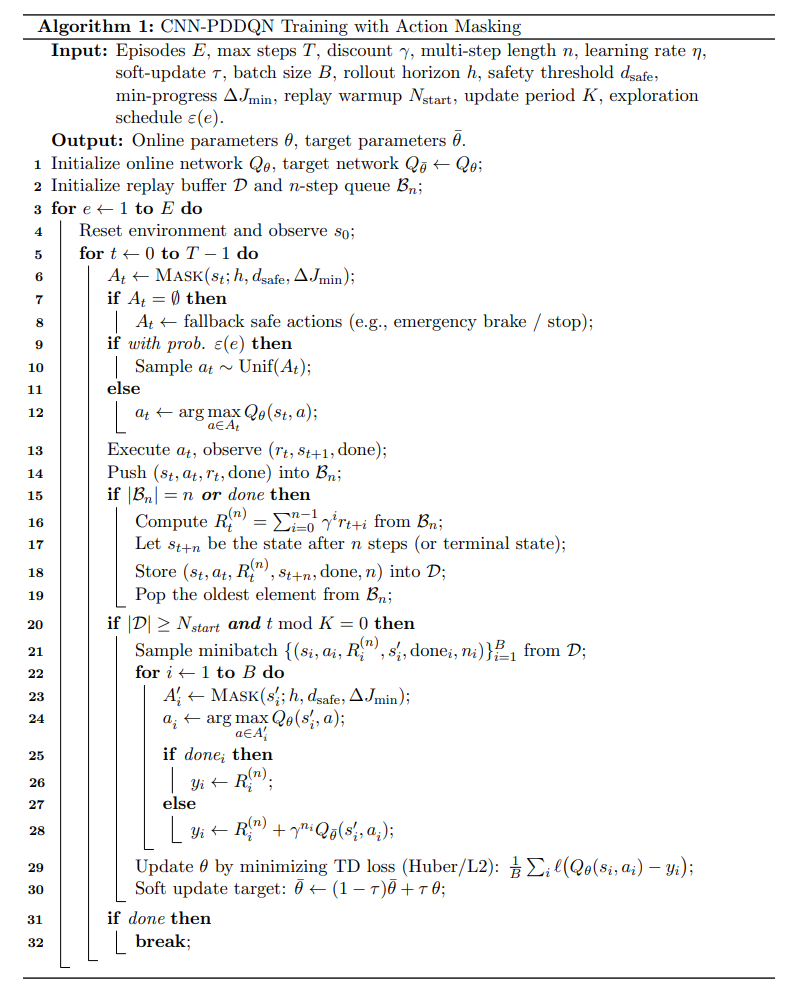
\includegraphics[width=0.88\columnwidth]{image7.png}
\caption{CNN-PDDQN训练与在线规划流程（伪代码）}
\label{fig:algorithm}
\end{figure}

% ══════════════════════════════════════════════════════════════
\section{结果与讨论}\label{sec:results}

为系统评估本文所提出方法的可行性与有效性，本文在PyCharm平台实现了所提算法及对比算法的统一仿真框架，并构建仿真森林环境开展对比测试。在相同起终点设置与一致的车辆运动学下，分别统计路径长度、平均绝对曲率与规划耗时等指标，并据此计算综合得分。随后将仿真结论与真实林地实验结果相结合，进一步验证所提方法相较基准算法的性能提升。

\subsection{基准算法}

为验证本文所提出方法的有效性与优越性，本文选取两类经典规划算法与多种强化学习基线进行对比：基于图搜索的Hybrid\,A*、基于采样的SS-RRT*，以及DQN系列强化学习算法（MLP/CNN两种网络结构）。

\subsubsection{混合A*}

Hybrid\,A*是面向非完整约束车辆的一类实用搜索规划算法，其核心思想是在连续状态空间$(x, y, \theta)$上进行A*搜索，但通过离散化航向角与采用满足车辆运动学来扩展节点，从而兼顾可行性与搜索效率。

\subsubsection{SS-RRT*}

RRT*是一种渐近最优的采样规划算法，通过随机采样扩展树结构，并逐步逼近最优解。由于原始RRT*生成的路径往往折线且不够平滑，面向车辆的常见做法是引入样条/曲线连接与连续碰撞检测。

\subsubsection{基准强化学习算法}

本文选取DQN系列作为强化学习基准。DQN以深度网络近似动作价值函数$Q(s,a)$，并采用经验回放与目标网络稳定训练，已被证明可在离散动作控制任务中取得良好效果。其TD目标一般写为：
\begin{equation}
  y = r + \gamma\max_{a'} Q(s', a'; \theta^-)
\end{equation}
为减轻DQN的过估计问题，引入Double\,DQN（DDQN），将``动作选择''与``动作评估''解耦：
\begin{equation}
  y^{\text{DDQN}} = r + \gamma Q_{\text{tgt}}\!\left(s', \arg\max_{a'} Q_{\text{online}}(s', a')\right)
\end{equation}

在网络结构方面，本文分别采用MLP（多层感知机）与CNN（卷积神经网络）进行价值函数逼近：MLP适合对低维特征进行非线性映射；CNN更擅长从栅格地图等空间输入中提取障碍分布与通道连通性等结构信息，从而提升对复杂场景的表达能力。

\subsection{评价指标}

为公平比较不同算法在同一环境下的运动规划性能，本文从轨迹几何质量与计算效率两个方面设置四项评价指标：路径长度$L$（m）、平均绝对曲率$\bar{\kappa}$（m$^{-1}$）、规划耗时$T$（s）以及综合得分$S$。

由于$L$、$\bar{\kappa}$与$T$的量纲与数值尺度不同，本文先对三项基础指标进行极差归一化，再计算综合得分。对任一指标$x \in \{L, \bar{\kappa}, T\}$，其归一化形式为：
\begin{equation}
  \tilde{x} = \frac{x - x_{\min}}{x_{\max} - x_{\min} + \varepsilon}
\end{equation}
其中$x_{\min}$与$x_{\max}$分别为同一测试集合内各对比算法该指标的最小值与最大值，$\varepsilon$为防止分母为零的极小常数。随后定义三项归一化指标的平均值：
\begin{equation}
  b = \frac{\tilde{L} + \tilde{\bar{\kappa}} + \tilde{T}}{3}
\end{equation}
并给出综合得分：
\begin{equation}
  S = 1 - b
\end{equation}
路径长度、平均绝对曲率与规划耗时均为越小越好的指标，而综合得分为越大越好。

\subsection{仿真场景下的对比验证}

为验证所提方法在森林场景中的有效性，本文在Python仿真平台构建随机森林环境，并在相同地图与一致的车辆运动学约束下，对所提方法与各基线算法进行对比测试。针对Hybrid\,A*与SS-RRT*等输出几何路径的传统规划器，为保证与学习型策略下公平比较，本文进一步引入模型预测控制（MPC）将离散路径转换为满足阿克曼车辆运动学与控制约束的可执行轨迹，从而统一轨迹生成与评价流程。

\subsubsection{长路径对比}

将训练完成的模型部署到随机森林仿真场景中进行测试。森林环境中树木半径随机、树间距随机；在该场景下随机生成10组起点与终点进行测试，图~\ref{fig:sim_long}展示了其中两次规划结果。

\begin{figure}[t]
\centering
\subfloat[(a)]{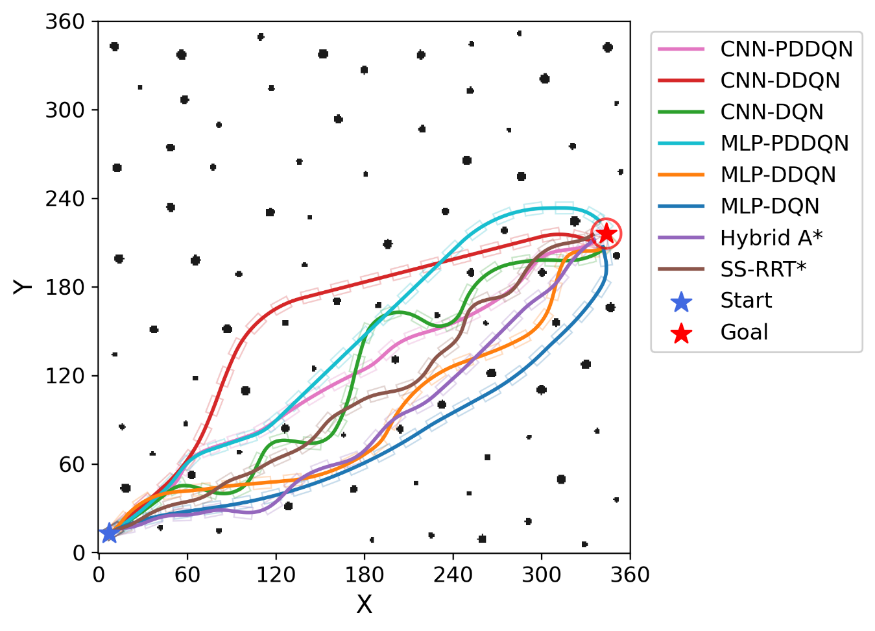
\includegraphics[width=0.48\columnwidth]{image8.png}}
\hfill
\subfloat[(b)]{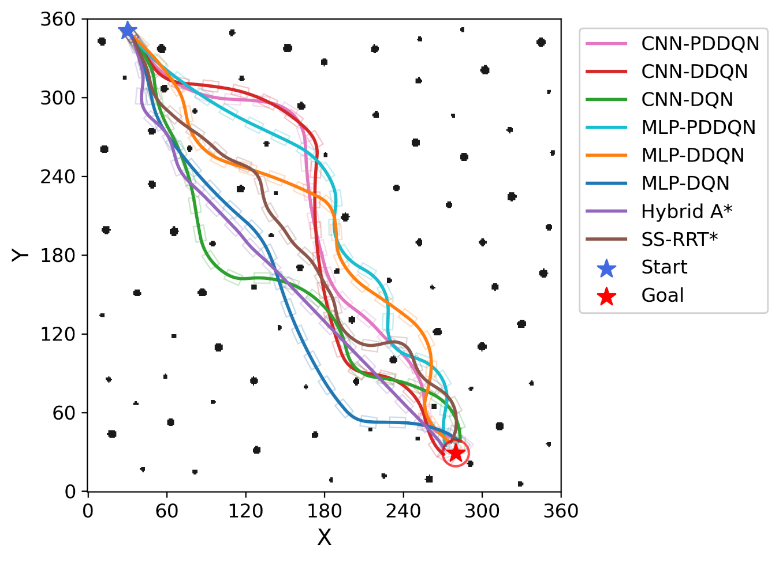
\includegraphics[width=0.48\columnwidth]{image9.png}}
\caption{随机森林仿真场景下长路径任务的规划结果对比示例}
\label{fig:sim_long}
\end{figure}

\begin{table}[t]
\centering
\caption{长路径任务中不同算法的平均性能指标对比}
\label{tab:long_path}
\footnotesize
\begin{tabular}{@{}lcccc@{}}
\toprule
\textbf{算法} & \textbf{路径(m)} & \textbf{曲率(1/m)} & \textbf{耗时(s)} & \textbf{得分} \\
\midrule
CNN-PDDQN  & \textbf{40.630} & 0.114 & 0.337 & \textbf{0.918} \\
CNN-DDQN   & 43.918 & 0.121 & 0.359 & 0.585 \\
CNN-DQN    & 44.397 & 0.137 & 0.353 & 0.505 \\
MLP-PDDQN  & 42.009 & 0.116 & 0.232 & 0.799 \\
MLP-DDQN   & 42.001 & 0.117 & 0.234 & 0.757 \\
MLP-DQN    & 42.775 & 0.104 & 0.246 & 0.737 \\
Hybrid A*  & 40.763 & \textbf{0.093} & 3.692 & 0.617 \\
SS-RRT*    & 40.923 & 0.191 & 2.316 & 0.273 \\
\bottomrule
\end{tabular}
\end{table}

\begin{figure}[t]
\centering
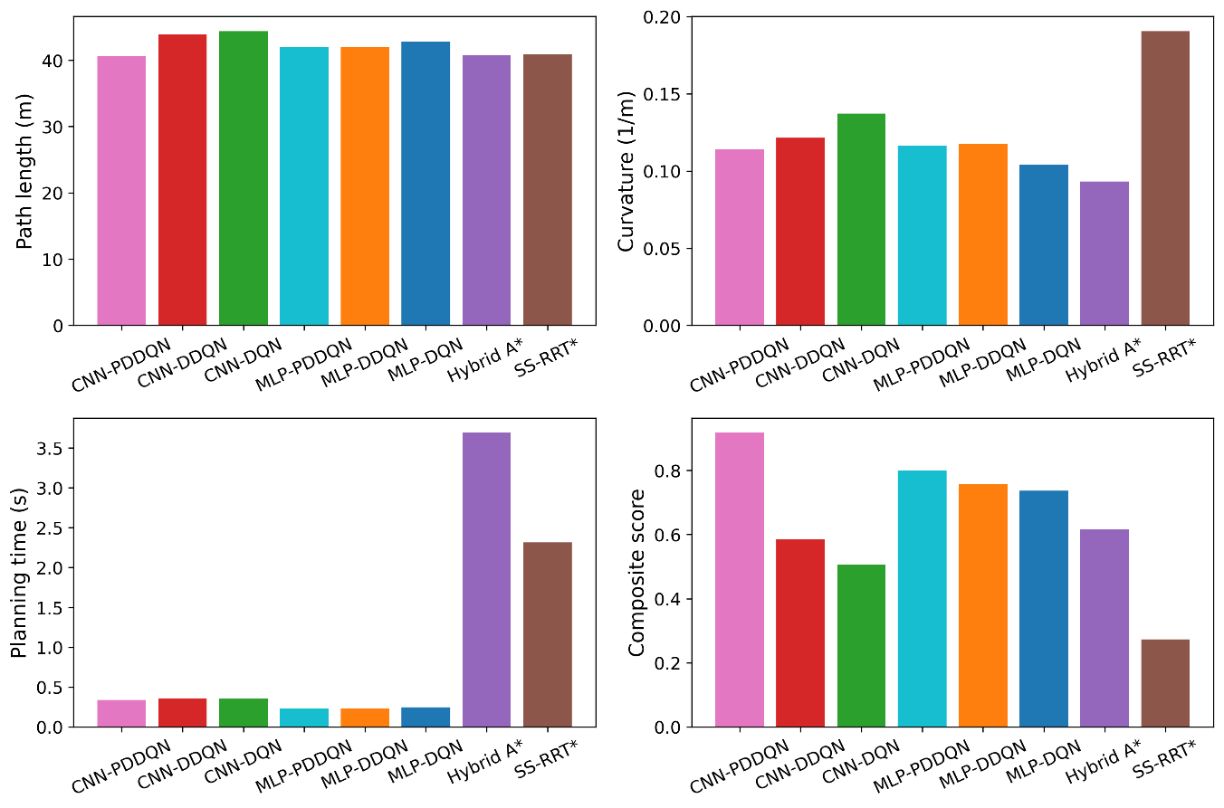
\includegraphics[width=\columnwidth]{image10.png}
\caption{长路径任务中不同算法的平均性能指标对比柱状图}
\label{fig:bar_long}
\end{figure}

表~\ref{tab:long_path}和图~\ref{fig:bar_long}展示了各算法在长路径任务上的平均指标。在CNN结构下，CNN-PDDQN（0.918）明显优于CNN-DDQN（0.585）与CNN-DQN（0.505），综合得分分别高出约56.9\%与81.8\%；同时路径长度也更短（40.630\,m vs 43.918\,m / 44.397\,m）。

在MLP结构下，MLP-PDDQN（0.799）优于MLP-DDQN（0.757）与MLP-DQN（0.737）。值得一提的是，MLP系列耗时更低（如MLP-PDDQN为0.232\,s），但其路径长度普遍更长（如42.009\,m），综合得分仍低于CNN-PDDQN（0.918），表明在该类森林非结构化场景中，CNN表征带来的局部环境理解能力对``走得更短、更稳、更可控''更关键。

\subsubsection{短路径对比}

进一步构造起终点距离更近的短路径任务，图~\ref{fig:sim_short}给出了两组典型结果，表~\ref{tab:short_path}和图~\ref{fig:bar_short}汇总了各算法在短路径任务上的平均指标。

\begin{figure}[t]
\centering
\subfloat[(a)]{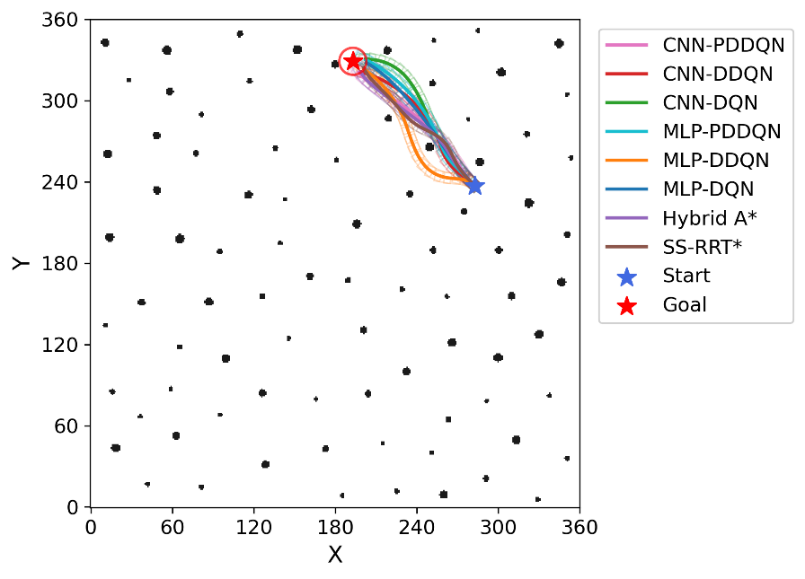
\includegraphics[width=0.48\columnwidth]{image11.png}}
\hfill
\subfloat[(b)]{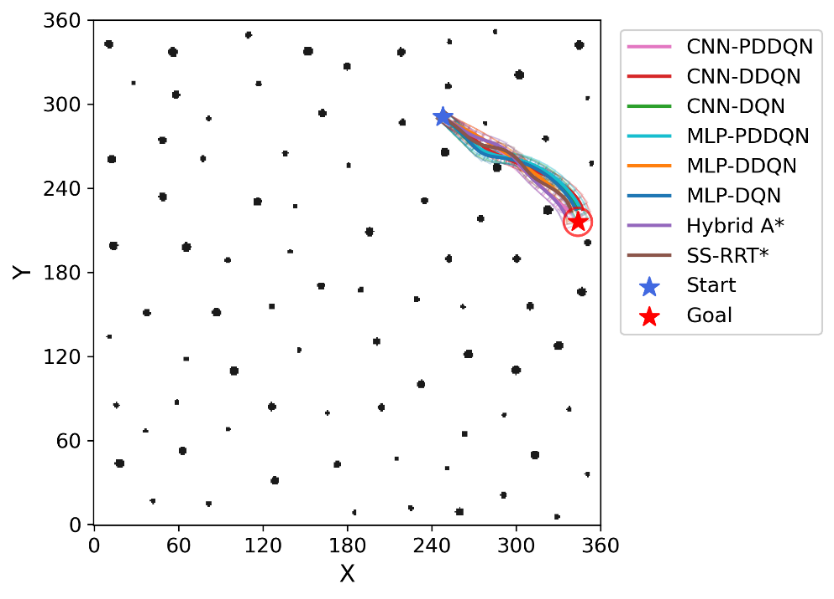
\includegraphics[width=0.48\columnwidth]{image12.png}}
\caption{随机森林仿真场景下短路径任务的规划结果对比示例}
\label{fig:sim_short}
\end{figure}

\begin{table}[t]
\centering
\caption{短路径任务中不同算法的平均性能指标对比}
\label{tab:short_path}
\footnotesize
\begin{tabular}{@{}lcccc@{}}
\toprule
\textbf{算法} & \textbf{路径(m)} & \textbf{曲率(1/m)} & \textbf{耗时(s)} & \textbf{得分} \\
\midrule
CNN-PDDQN  & \textbf{40.630} & 0.114 & 0.337 & \textbf{0.918} \\
CNN-DDQN   & 43.918 & 0.121 & 0.359 & 0.585 \\
CNN-DQN    & 44.397 & 0.137 & 0.353 & 0.505 \\
MLP-PDDQN  & 42.009 & 0.116 & 0.232 & 0.799 \\
MLP-DDQN   & 42.001 & 0.117 & 0.234 & 0.757 \\
MLP-DQN    & 42.775 & 0.104 & 0.246 & 0.737 \\
Hybrid A*  & 40.763 & \textbf{0.093} & 3.692 & 0.617 \\
SS-RRT*    & 40.923 & 0.191 & 2.316 & 0.273 \\
\bottomrule
\end{tabular}
\end{table}

\begin{figure}[t]
\centering
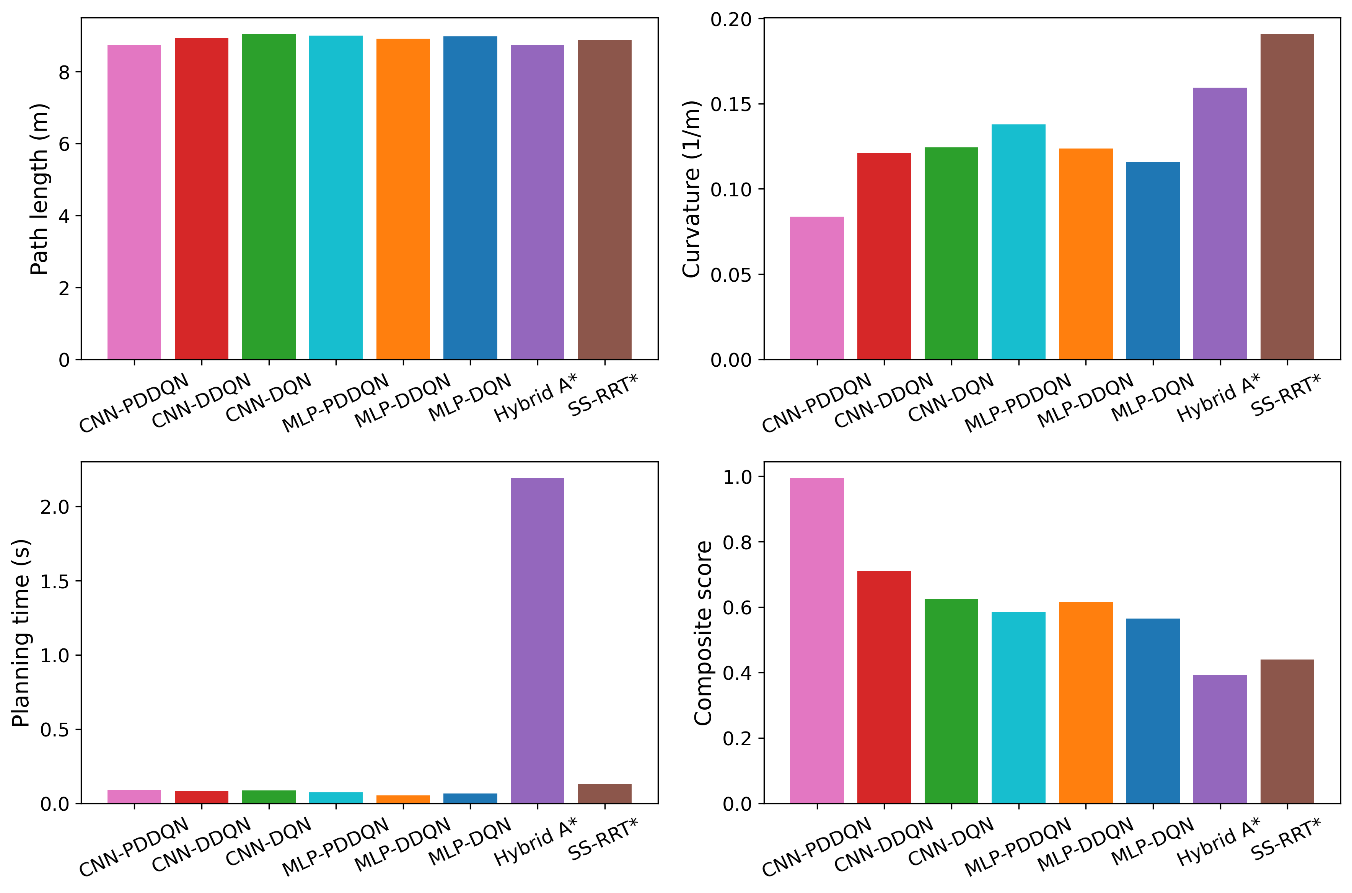
\includegraphics[width=\columnwidth]{image13.png}
\caption{短路径任务中不同算法的平均性能指标对比柱状图}
\label{fig:bar_short}
\end{figure}

从表~\ref{tab:short_path}可见，CNN-PDDQN在短路径任务中同样取得最高综合得分（0.918），并在规划耗时（0.337\,s）、路径长度（40.630\,m）与曲率（0.114\,1/m）等指标上保持良好平衡；传统方法Hybrid\,A*与SS-RRT*仍然受到规划耗时较高（3.692\,s / 2.316\,s）或曲率偏大（SS-RRT*为0.191\,1/m）的影响，综合得分明显偏低（0.617 / 0.273）。

\subsection{真实场景下的对比验证}

\subsubsection{真实场景的建立}

为验证所提方法在真实林地环境中的可行性与泛化能力，在中国黑龙江省哈尔滨市东北林业大学森林试验场建立真实场景的先验点云地图，如图~\ref{fig:realmap_site}所示。

\begin{figure}[t]
\centering
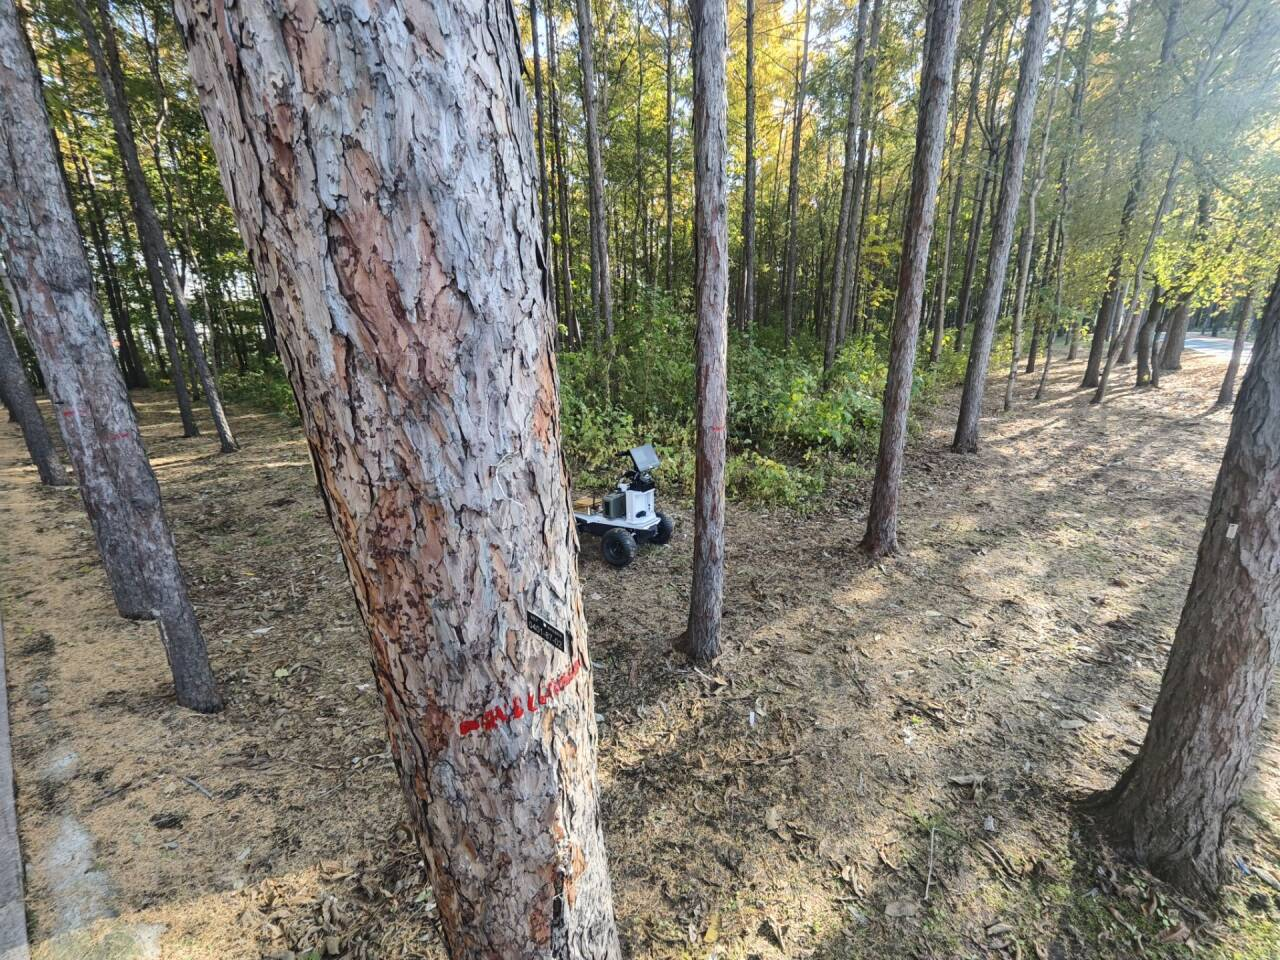
\includegraphics[width=0.6\columnwidth]{image14.png}
\caption{真实林地试验场景}
\label{fig:realmap_site}
\end{figure}

按照第~\ref{sec:method}节所述流程，采用FAST-LIO2融合激光雷达与IMU数据构建三维点云先验地图，并对地图进行体素降采样与统计离群点移除（SOR）滤波，结果如图~\ref{fig:pointcloud}所示。

\begin{figure}[t]
\centering
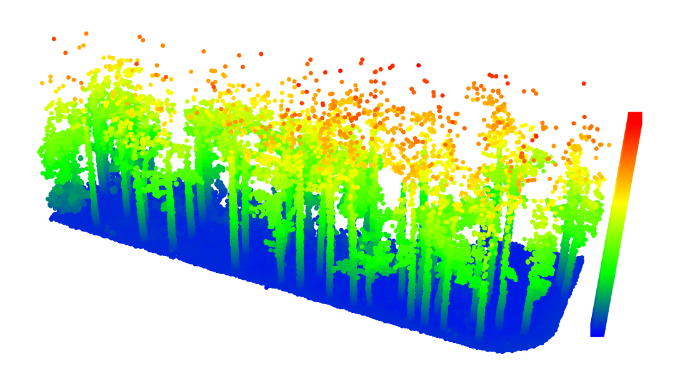
\includegraphics[width=0.85\columnwidth]{image15.png}
\caption{FAST-LIO2构建后降采样与SOR滤波后的三维点云先验地图}
\label{fig:pointcloud}
\end{figure}

在点云先验地图基础上，采用第~\ref{sec:method}节提出的可通行性评估对点云进行分割，得到不可通行点云，并将分割结果投影生成二维占据栅格地图，如图~\ref{fig:traversability}所示。栅格地图分辨率为0.1\,m，其中黑色表示障碍物/不可通行区域，白色表示可通行区域。由图~\ref{fig:traversability}可见，树干等静态障碍以及坡度较大的区域均被正确标记为不可通行，从而为后续运动规划提供可靠的可行域约束。

\begin{figure}[t]
\centering
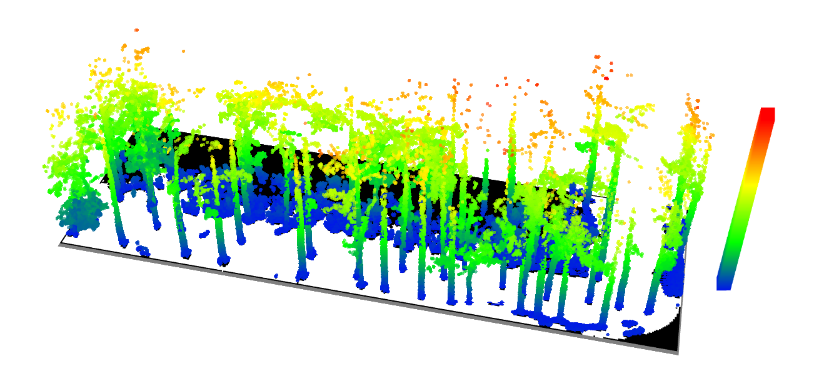
\includegraphics[width=0.85\columnwidth]{image16.png}
\caption{可通行性分割结果及带点云的栅格地图}
\label{fig:traversability}
\end{figure}

\subsubsection{真实场景下的结果}

在上述地图与车辆运动学约束条件下，将CNN-PDDQN与多种基线算法（DQN系列、Hybrid\,A*、SS-RRT*）在相同起终点条件下进行对比测试。对每次规划记录路径长度、平均绝对曲率与规划耗时，并按第~\ref{sec:results}节定义计算综合得分。图~\ref{fig:real_paths}给出了代表性轨迹结果，表~\ref{tab:real_results}和图~\ref{fig:bar_real}汇总了各算法的平均性能指标。

\begin{figure*}[t]
\centering
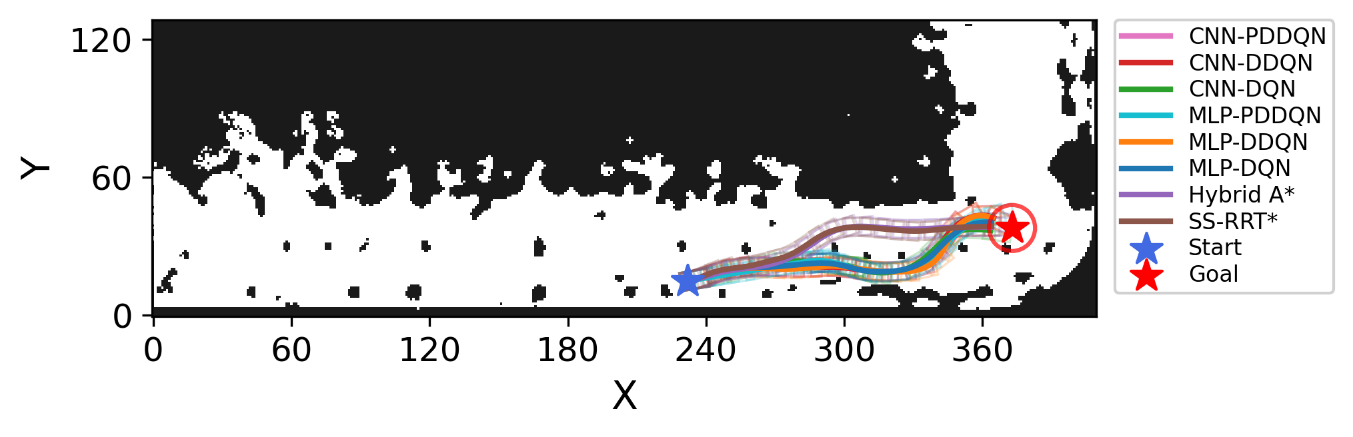
\includegraphics[width=\textwidth]{image17.png}
\caption{真实林地场景下路径规划算法对比}
\label{fig:real_paths}
\end{figure*}

\begin{table}[t]
\centering
\caption{真实林地实验中不同算法的平均性能指标对比}
\label{tab:real_results}
\footnotesize
\begin{tabular}{@{}lcccc@{}}
\toprule
\textbf{算法} & \textbf{路径(m)} & \textbf{曲率(1/m)} & \textbf{耗时(s)} & \textbf{得分} \\
\midrule
CNN-PDDQN  & 15.730 & 0.221 & 0.185 & \textbf{1.085} \\
CNN-DDQN   & 15.730 & 0.221 & 0.186 & 1.085 \\
CNN-DQN    & 17.311 & 0.180 & 0.243 & 0.813 \\
MLP-PDDQN  & 18.119 & 0.227 & 0.173 & 0.673 \\
MLP-DDQN   & 16.886 & 0.175 & \textbf{0.134} & 0.447 \\
MLP-DQN    & \textbf{15.704} & \textbf{0.150} & 0.184 & 0.247 \\
Hybrid A*  & 16.655 & 0.103 & 2.361 & 0.376 \\
SS-RRT*    & 16.756 & 0.130 & 1.891 & 0.404 \\
\bottomrule
\end{tabular}
\end{table}

\begin{figure}[t]
\centering
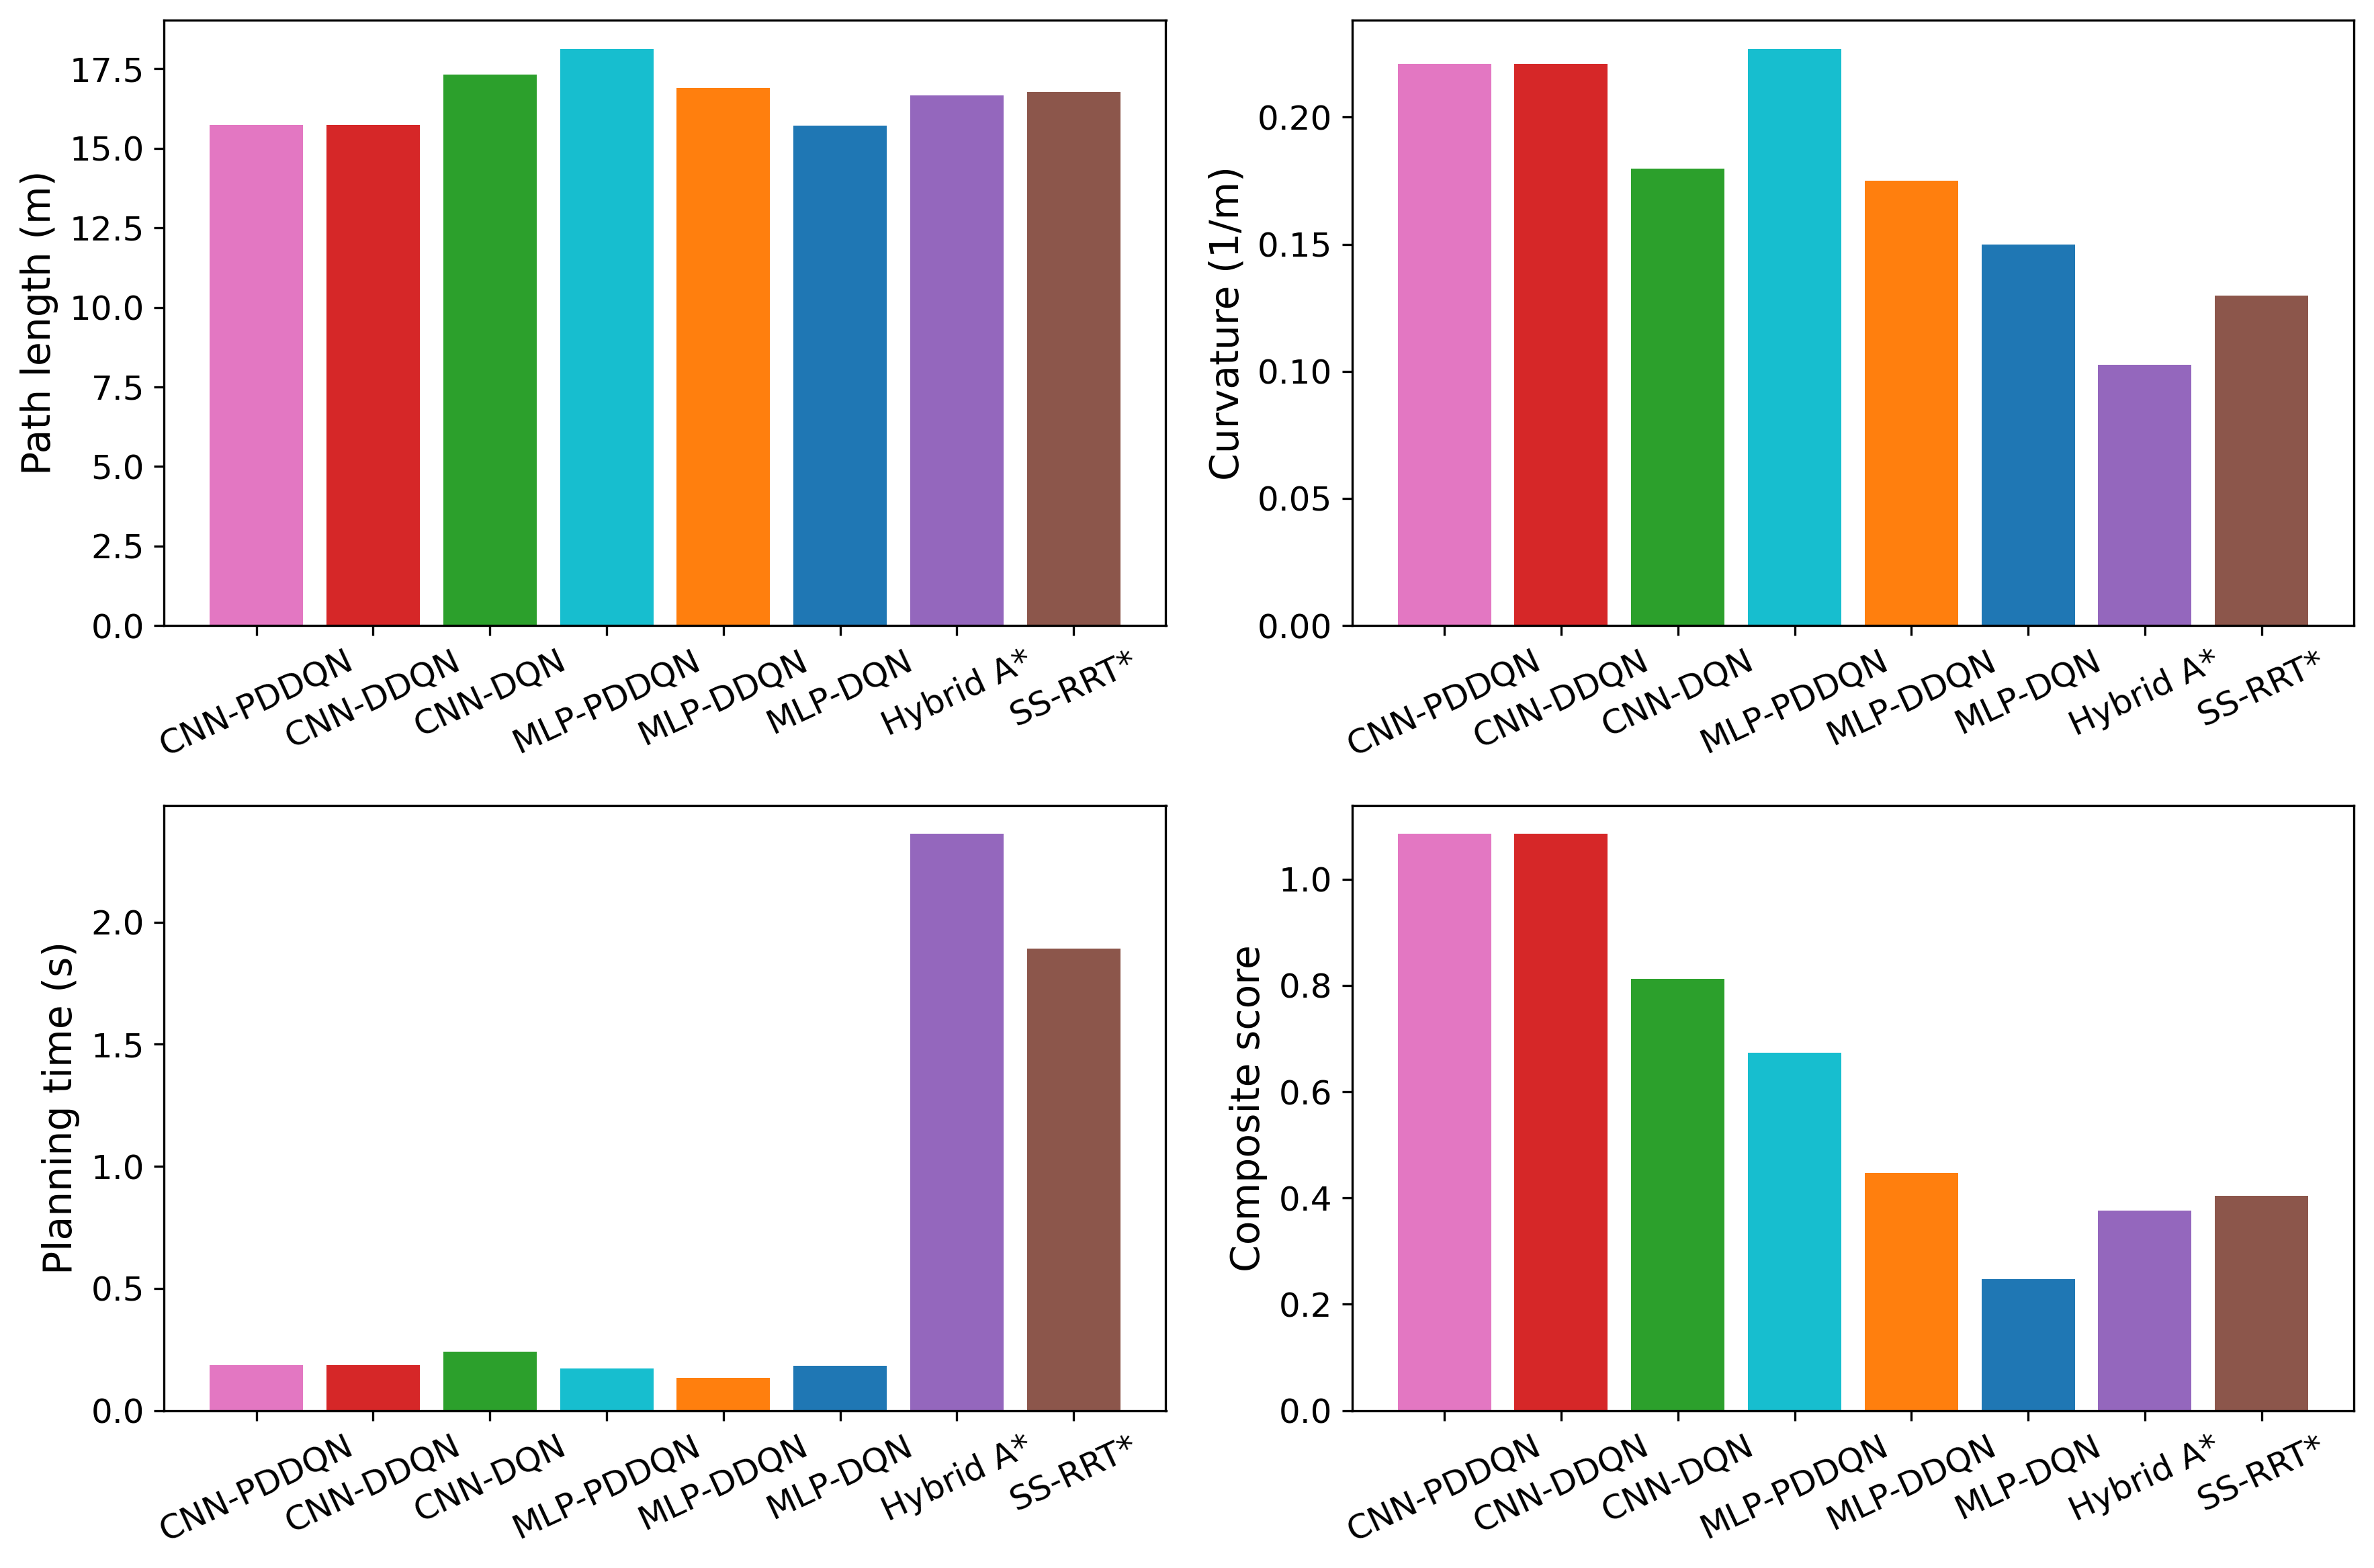
\includegraphics[width=\columnwidth]{image18.png}
\caption{真实林地实验中不同算法的平均性能指标对比柱状图}
\label{fig:bar_real}
\end{figure}

从表~\ref{tab:real_results}可见，CNN-PDDQN在真实林地场景中取得最高综合得分（1.085），规划耗时为0.185\,s，相较Hybrid\,A*（2.361\,s）与SS-RRT*（1.891\,s）具有明显实时性优势。在路径长度与平均绝对曲率指标上，CNN-PDDQN与其他学习型基线保持同量级水平，能够在狭窄通道内生成可执行轨迹。传统规划方法虽然曲率相对更小，但规划开销较大，导致在线规划耗时显著上升。

% ══════════════════════════════════════════════════════════════
\section{结论}\label{sec:conclusion}

在树干密集、通道狭窄且地形起伏的森林非结构化环境中，为阿克曼式地面无人车（UGV）实现满足运动学约束的实时、安全、可执行路径规划，是提升森林巡检与作业自主化水平的关键。然而，该类环境同时带来多重挑战：三维点云到可通行区域的评估与表达难度大；狭窄通道下传统图搜索/采样规划计算开销高；以及非完整约束与安全裕度共同作用下的可控性与稳定性难以兼顾。为此，本文提出一种面向森林场景的深度强化学习运动规划方法，融合先验三维建图、可通行性评估与约束感知策略学习，以实现实时、稳定且可执行的在线规划。

本研究的主要贡献如下：

\begin{enumerate}
  \item 构建了基于FAST-LIO2的先验点云建图与可通行性评估流程，实现点云分割并生成栅格地图，为后续规划提供可靠的先验地图。
  \item 将规划过程建模为马尔可夫决策过程，设计CNN-PDDQN价值网络，并结合进度、时间、平滑/可控性与双圆足迹安全裕度构造奖励函数，使学习策略能够在狭窄通道中生成更短、更稳的可执行路径。
  \item 提出推理阶段的约束感知机制，引入在线动作掩码与短视滚动预测的可行域过滤，并配合回退机制与分层验证，减少必碰撞/低收益动作选择与振荡风险，提升在线规划稳定性。
  \item 在随机森林仿真与真实林地场景中进行了充分对比验证，系统评估了路径长度、曲率与规划耗时等指标，证明所提方法在路径质量与规划效率之间取得更优折中。
\end{enumerate}

该方法已在仿真与实地实验中得到验证：能够在复杂林地环境中高效识别可通行区域，并快速生成满足阿克曼运动学约束的安全可执行轨迹。在仿真长路径任务中平均规划耗时为0.337\,s、综合得分为0.918；在真实林地场景中平均规划耗时为0.185\,s、综合得分为1.085，均明显优于Hybrid\,A*与SS-RRT*等传统方法的实时性表现。

\ack{[TODO: 致谢相关人员、机构和资金支持（可注明课题编号和资助方）]}

\section*{利益冲突声明}

作者声明不存在可能影响本文所报告工作的已知竞争性财务利益或个人关系。

% ══════════════════════════════════════════════════════════════
\bibliographystyle{unsrt}
\bibliography{references}

\end{document}
